\documentclass[conference]{IEEEtran}

\usepackage{cite}
\usepackage{amsmath,amssymb,amsfonts}
\usepackage{graphicx}
\usepackage{textcomp}
\usepackage{xcolor}
\usepackage{booktabs}
\usepackage{balance}
\usepackage{url}

\title{Dimension-Controlled Linear Probing of Fashion-MNIST Convolutional Networks}

\author{\IEEEauthorblockN{Hendrik Strauss}
\IEEEauthorblockA{Introduction to Deep Learning\\
Universit\"at Osnabr\"uck\\
\relax[hestrauss@uni-osnabrueck.de]}}

\begin{document}
\maketitle

\begin{abstract}
Classifier accuracy does not reveal which distinctions are linearly accessible
in a network's hidden representations. Using Fashion-MNIST and frozen linear
probes, I test whether footwear and tops, groupings absent from ten-class CNN
training, can be recovered with few labels. Pixels, random CNN features, and
trained activations are compared after matched Gaussian projection to 32
dimensions, across budgets of 10--200 images and 50 matched runs. With only 10
labels, trained FC features reached macro-F1 scores of $0.9803$ for footwear
and $0.9263$ for tops, outperforming both baselines. Random features were
nonetheless informative, especially for footwear. A second experiment compares
ten-class supervision with footwear/non-footwear and tops/non-tops objectives.
Coarse training made aligned boundaries highly accessible but did not
consistently improve internal distinctions over random features, performing
worse for footwear and only slightly better for tops; fine-label features
remained strongest. Thus, in this setting, fine-label training exposed broader
groupings not directly supervised, whereas coarse objectives offered no
consistent benefit for their internal structure.
\end{abstract}

\begin{IEEEkeywords}
linear probes, representation learning, sample efficiency, Fashion-MNIST,
convolutional neural networks
\end{IEEEkeywords}

\section{Introduction}
Convolutional neural networks are normally evaluated through the accuracy of
their final classifier. This leaves a more diagnostic question unanswered:
what information is already available to a simple downstream learner at each
hidden layer? Linear probes attempt this question by fitting an independent
linear classifier to frozen activations, without changing the network itself
\cite{alain2016}. A high probe score indicates that a target concept is
linearly accessible, although it does not prove that the CNN's own classifier
uses that concept.

Fashion-MNIST contains 70,000 grayscale $28\!\times\!28$ images in ten clothing
classes, with an official split of 60,000 training and 10,000 test images
\cite{xiao2017}. Though not natively provisioned, its low level labels quite conveniently support grouping at a more general semantic level: for
example, sandal, sneaker, and ankle boot form a footwear superclass, while
T-shirt/top, pullover, coat, and shirt form a tops superclass. This makes it a
useful testbed for studying how supervised objectives can shape representations.
Fashion-MNIST therefore provides a compact setting in which to study the decodability of broader semantic categories. We use raw pixels as a baseline for how accessible these categories are in the input itself. Because even randomly initialized CNNs can produce useful features \cite{xue2018}, we additionally compare random and trained CNN representations to distinguish the contribution of the architecture from that of supervised learning.

This project asks two questions. First, can superclass distinctions absent from
CNN training be decoded from its hidden layers using only a few probe labels,
and where are they most accessible? Second, does explicit superclass training
also improve distinctions within that superclass, or does it primarily
strengthen the trained boundary? Experiment 1 probes footwear and tops
throughout a ten-class CNN, using pixels and a random CNN as baselines.
Experiment 2 compares ten-class supervision with footwear/non-footwear and
tops/non-tops supervision. All comparisons use matched labeled examples and a
common 32-dimensional feature budget.

\section{Methods}
\subsection{Data, Architecture, and Training}
Pixels were scaled to $[0,1]$ without augmentation. A stratified split assigned
50,000 official training images to CNN fitting and 10,000 to validation. The
official 10,000-image test set was held out until all models and probes had
been selected. The CNN contains two \(3\times3\) convolutional layers, producing 16 and 32 feature maps, respectively. Each uses ReLU and $2\!\times\!2$ max pooling, followed by a
128-unit ReLU layer and a classifier. Flattened activation dimensions are
3,136 (Conv1), 1,568 (Conv2), and 128 (FC).

Models were trained for 10 epochs with cross-entropy loss, Adam, learning rate
$10^{-3}$, and batch size 64. The checkpoint with the lowest validation loss
was retained. All reported probes used one seed-42 realization of each CNN condition. Each probe condition was evaluated using ten labeled-data samples with and five Gaussian random projections, yielding 50 matched runs. Reported means and standard deviations therefore reflect variation in probe sampling and projection, not variation across CNN training runs. The main model was trained on the original ten Fashion-MNIST classes. In the extension, the random, fine-label, and coarse-label networks began with identical shared the same initial feature-extractor weights. The fine-label network  was trained on the ten original classes, whereas the coarse-label network predicted footwear (classes 5, 7, and 9) versus non-footwear.

\subsection{Dimension-Controlled Linear Probes}
I compared raw pixels and frozen Conv1, Conv2, and FC activations from random
and trained CNNs. Every representation was mapped to 32 dimensions by a fixed
Gaussian random projection. Random and trained representations from the same
layer received identical projection matrices. Five projection seeds (0-4)
were crossed with ten nested sampling repeats (sampling seeds 42-51).

L2-regularized logistic regressions were trained with exact total label
budgets $n\in\{10,20,30,50,80,110,150,200\}$. Extracted representations were standardized feature-wise using statistics computed exclusively on the probe-training split and then applied unchanged to the validation and test splits. The inverse regularization strength
$C\in\{0.01,0.1,1\}$ was selected by macro-F1 on a fixed 2,000-image validation
subset. All probe models were fitted and serialized before test-set evaluation. For each task and representation condition, results report the mean and sample standard deviation over the 50 matched sampling/projection runs.

The main tasks in Experiment 1 were binary footwear and tops recognition.
Samples were nested and stratified over all ten original classes. Experiment 2
evaluated footwear and tops separately, using seven and eleven task-specific
probes, respectively. For each superclass, these comprised one multiclass
task, all pairwise contrasts, and one class-versus-non-superclass task per
class. Training examples were distributed as evenly as possible across the target classes. Macro-F1 was the
primary metric; accuracy, balanced accuracy, per-class F1, and confusion
matrices were also stored. Split indices, checkpoint hashes, environment
metadata, raw results, and fitted probe bundles are retained for
reproducibility; code and artifacts will be published at
\url{[PUBLIC-GITLAB-URL]}.

\section{Results and Discussion}
\subsection{Experiment 1: Layer-Wise Sample Efficiency}

The ten-class CNN showed mild overfitting. Training accuracy increased from
$0.9155$ at the selected epoch 6 to $0.9361$ at epoch 10, while validation loss
was lowest at epoch 6 ($0.2499$) and did not improve thereafter. Checkpoint
selection therefore avoided using the later, more overfit model.

Fig.~\ref{fig:main} shows that learned representations were most beneficial
when labels were scarce. With only 10 probe-training images, trained FC
features achieved $0.9803\pm0.0192$ macro-F1 for footwear, compared with
$0.9168\pm0.0521$ for random FC features and $0.8754\pm0.0627$ for pixels. For
tops, the corresponding scores were $0.9263\pm0.0223$, $0.7808\pm0.0595$, and
$0.7837\pm0.0424$. At 200 labels, trained FC features remained strongest,
reaching $0.9974$ for footwear and $0.9625$ for tops.

\begin{figure*}[t]
    \centering
    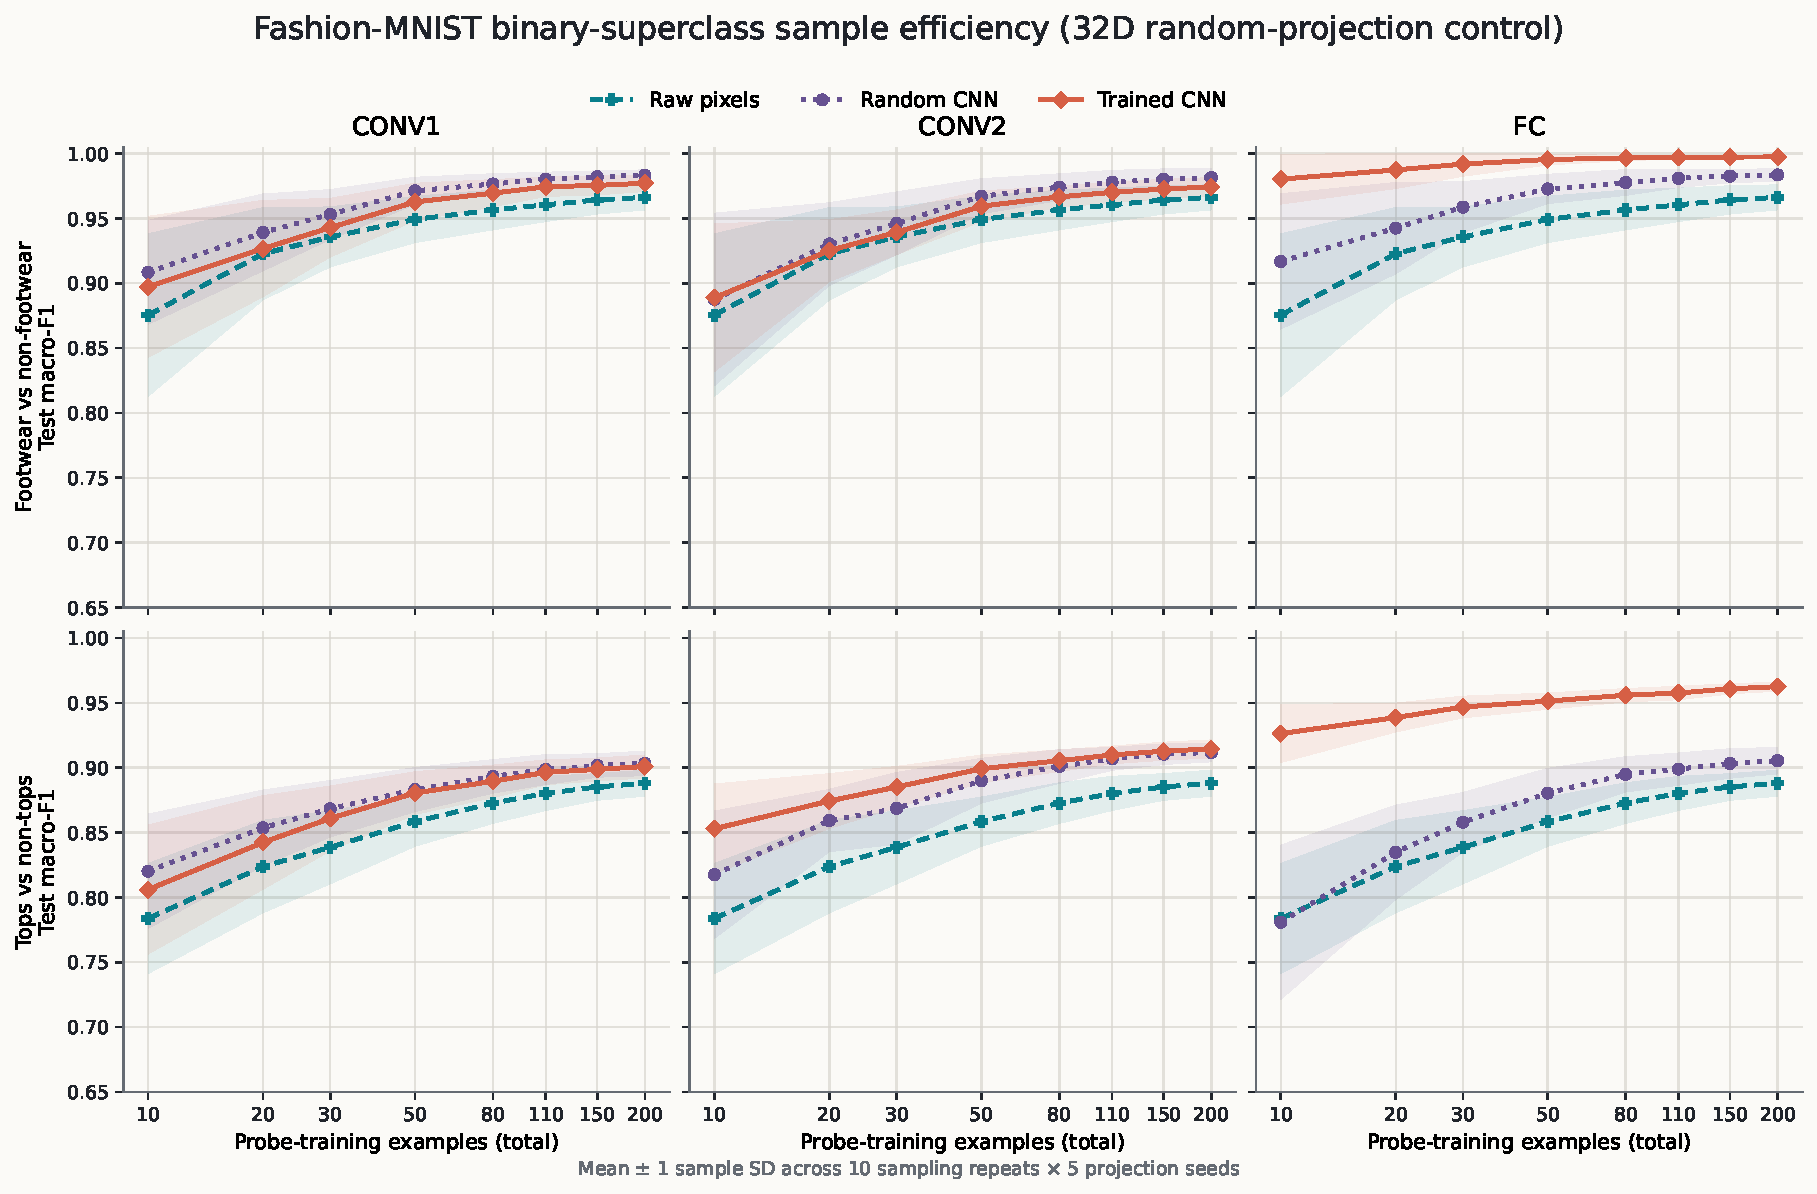
\includegraphics[width=0.76\textwidth]{figures/main_sample_efficiency.pdf}
    \caption{Test macro-F1 as a function of the exact total probe-training
    budget. Lines show means and shaded regions show one sample standard
    deviation across 10 nested sampling repeats and five matched 32D Gaussian
    projections. The random CNN is a strong control, but supervised features,
    especially FC features, are more sample-efficient.}
    \label{fig:main}
\end{figure*}

The strong random-CNN baseline suggests that the convolutional architecture contributes to the gain over pixels. Even without training, convolution encodes locality, while ReLU and pooling produce nonlinear features with some tolerance to small translations. Mapping every representation to 32 dimensions prevents feature count alone from explaining the differences. Nevertheless, trained FC features performed best across all label budgets, with the largest advantages at low \(n\) and for tops. This pattern is consistent with supervised learning making task-relevant distinctions more linearly accessible


\subsection{Experiment 2: Training Objective Shapes Transfer}
Experiment 2 asked whether learning a coarse superclass boundary also improves
distinctions within that superclass. It did not do so consistently. At 200
labels, coarse FC was below random FC on three-way footwear
($0.8505$ versus $0.8635$) and averaged slightly lower across the footwear
pairwise contrasts ($0.9200$ versus $0.9278$). For tops, however, coarse FC
exceeded random FC on the four-way task ($0.6185$ versus $0.5771$) and across
the pairwise contrasts ($0.8375$ versus $0.8174$). This difference may reflect
that tops-versus-non-tops was the harder coarse task ($0.9809$ versus $0.9992$
test accuracy), requiring richer features that also preserved more
within-superclass structure. Fine-label FC remained substantially stronger on
both multiway tasks, reaching $0.9585$ for footwear and $0.7973$ for tops.

As expected, coarse FC performed strongly on the aligned
class-versus-non-superclass probes. With only 10 labels, it averaged $0.9942$
for footwear and $0.9392$ for tops, compared with $0.9401$ and $0.8799$ for
fine FC. This boundary advantage is unsurprising; the more informative result
is that transfer within the superclass was category-dependent and could fall
below the untrained baseline. Fig.~\ref{fig:extension} summarizes both effects.

\begin{figure*}[!t]
    \centering
    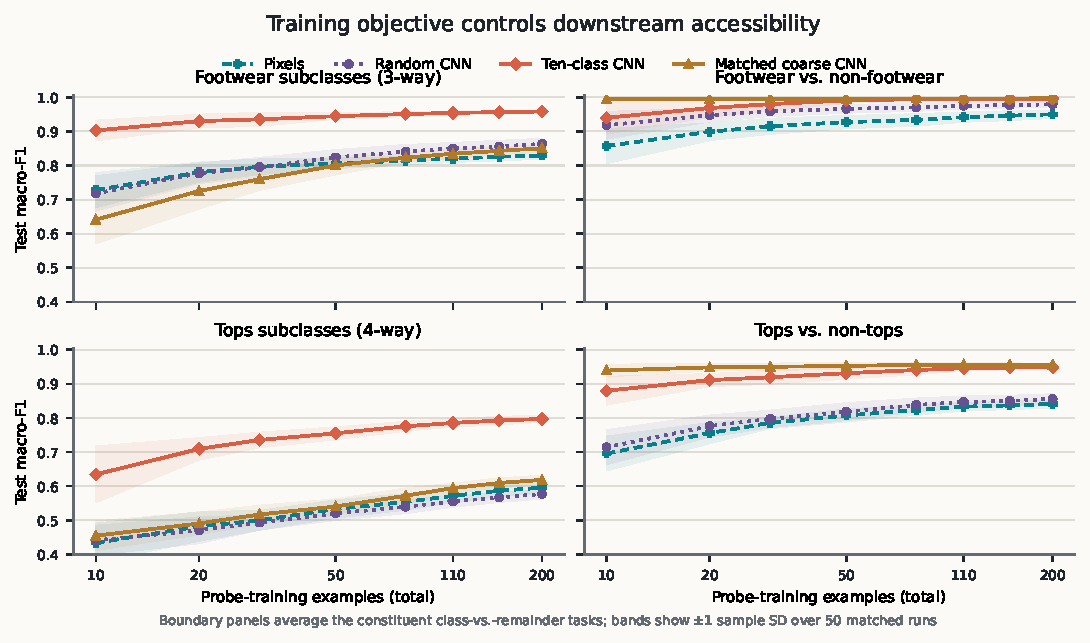
\includegraphics[width=0.68\textwidth]
        {figures/extension_objective_four_panel.pdf}
    \caption{Experiment 2, using 32D FC features. Rows show footwear and tops;
    columns show within-superclass decoding and the corresponding superclass
    boundary. Lines and shaded regions show mean $\pm$ one sample standard
    deviation over the same 50 matched runs as Experiment 1.}
    \label{fig:extension}
\end{figure*}

\subsection{Limitations}

The analysis uses one seed-42 training run per CNN condition; the 50 probe runs
therefore capture sampling and projection variability, not variation across
learned backbones. Fashion-MNIST is small and visually regular, and near-ceiling
performance on several superclass-boundary tasks may obscure differences
between representations. Linear probes measure only linear accessibility, while
random projection may distort representations differently despite equalizing
their dimensionality. Replication across training seeds, architectures, and a
more challenging natural-image dataset would provide a stronger generalization
test.

\section{Conclusion}

Experiment 1 showed that footwear and tops, although absent from the ten-class
objective, were decodable with only 10 probe labels and most accessible at FC.
Random features were informative, but trained FC features performed best,
especially for tops. Experiment 2 showed that coarse training learned its
target boundary but did not consistently improve internal distinctions over
random features, performing worse for footwear and only slightly better for
tops.

\begin{thebibliography}{00}
\bibitem{xiao2017}
H. Xiao, K. Rasul, and R. Vollgraf, \emph{Fashion-MNIST: A novel image dataset
for benchmarking machine learning algorithms}, arXiv:1708.07747, 2017.

\bibitem{alain2016}
G. Alain and Y. Bengio, \emph{Understanding intermediate layers using linear
classifier probes}, arXiv:1610.01644, 2016.

\bibitem{xue2018}
Y. Xue and U. Roshan, \emph{Image classification and retrieval with random
depthwise signed convolutional neural networks}, arXiv:1806.05789, 2018.
\end{thebibliography}

\end{document}
